\documentclass[11pt,a4paper]{article}

% Packages
\usepackage[margin=2.5cm]{geometry}
\usepackage{graphicx}
\usepackage{enumitem}
\usepackage{hyperref}
\usepackage{titlesec}
\usepackage{tikz}
\usepackage[table]{xcolor}
\usepackage{makecell}
\usepackage{booktabs}


\setlist[itemize]{noitemsep, topsep=0pt}
\usetikzlibrary{positioning, calc, arrows.meta}
\setlength{\parskip}{0.8em}

% Compact section spacing
\titlespacing*{\section}{0pt}{0.3em}{0.3em}
\titlespacing*{\subsection}{0pt}{0.4em}{1pt}

\renewcommand{\arraystretch}{1.3} % increases vertical spacing

%---------------------------
\begin{document}

\begin{center}
    {\LARGE \textbf{ENG4200 Coursework 1 Report}}\\[0.5em]
    \textbf{Student Name:} {Elsie Msalila} \quad 
    \textbf{ID:} {2778939M} \\[0.5em]
    Dataset: {Predict Age Abalones}
\end{center}

%---------------------------------------
\section{Objective}
The aim of this project is to understand the structure of regression pipelines in scikit-learn and evaluate their effectiveness. The chosen dataset is the Predict Age Abalones dataset which uses physical properties of samples to predict their age. Each sample has eight input features such as height, length, diameter, and weight, as well as one target variable - the number of rings (which correlates to their age).

In this project two different regression models - Linear and Ridge regression - were applied to the chosen dataset. The results of each of these models were then compared and the effectiveness of each model was commented on.

%---------------------------------------
\section{Pipeline Design}

\begin{figure}[h!]
    \begin{center}
        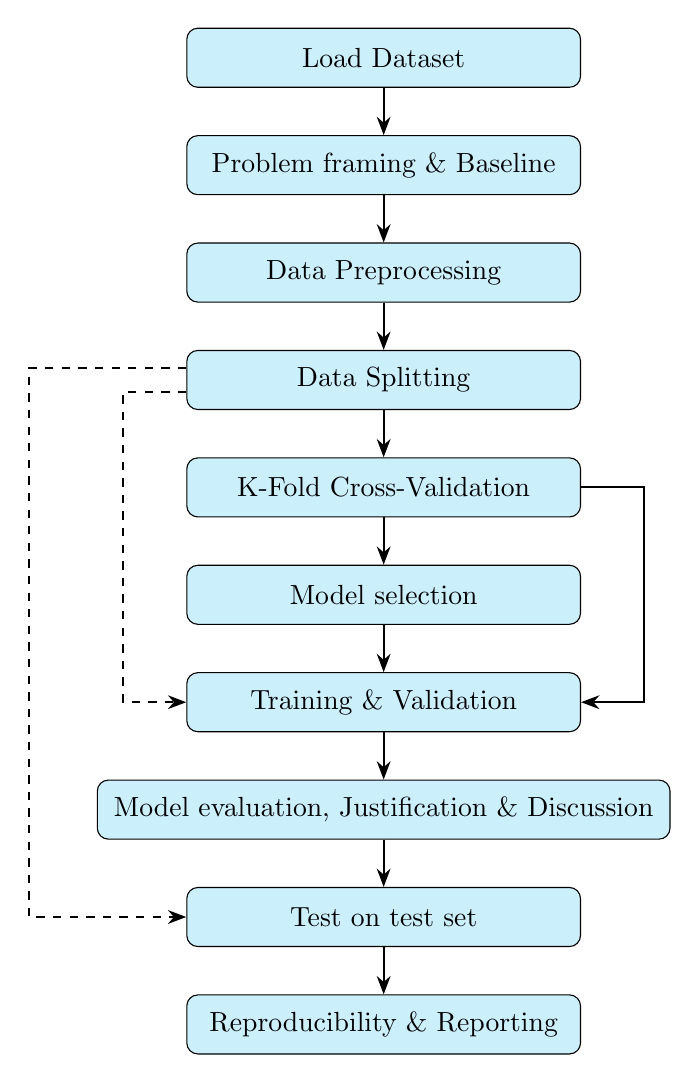
\begin{tikzpicture}[node distance=0.6cm, every node/.style={rectangle, draw, rounded corners, align=center, minimum width=5cm, minimum height=0.75cm, inner sep=6pt, fill=cyan!20}, >=Stealth]
        % Nodes
        \node (id1) {Load Dataset};
        \node (id2) [below=of id1] {Problem framing \& Baseline};
        \node (id3) [below=of id2] {Data Preprocessing};
        \node (id4) [below=of id3] {Data Splitting};
        \node (id5) [below=of id4] {K-Fold Cross-Validation};
        \node (id6) [below=of id5] {Model selection};
        \node (id7) [below=of id6] {Training \& Validation};
        \node (id8) [below=of id7] {Model evaluation, Justification \& Discussion};
        \node (id8_5) [below=of id8] {Test on test set};
        \node (id9) [below=of id8_5] {Reproducibility \& Reporting};

        % Main vertical arrows
        \foreach \i/\j in {id1/id2, id2/id3, id3/id4, id4/id5, id5/id6, id6/id7, id7/id8, id8/id8_5, id8_5/id9}
        \draw[->, thick] (\i) -- (\j);

        % Output arrows
        \draw[->, thick] (id5.east) -- ++(0.8,0) |- (id7.east);
        \draw[->, thick, dashed] ([yshift=-0.15cm] id4.west) -- ++(-0.8,0) |- (id7.west);
        \draw[->, thick, dashed] ([yshift=0.15cm] id4.west) -- ++(-2,0) |- (id8_5.west);

        \end{tikzpicture}
    \end{center}
    \caption{Pipeline Design}
    \label{fig:pipeline}
\end{figure}

\subsection{Problem Framing}
The target variable chosen for prediction is the number of rings, as this directly correlates with the age of the abalones. Since this is a continuous variable rather than categoric, regression techniques were selected for this task. 

\subsection{Data Pre-processing}
Once the dataset was loaded, it was checked for any missing or invalid values. Upon inspection, it was found that the dataset did not contain any missing values. However, the minimum value for height was zero, which is not physically possible for abalones. The dataset was searched for zero height instances and it was found that there were two rows with this issue. Due to the small number of affected rows, they were removed from the dataset as they have minimal impact on the overall data distribution, representing only 0.05\%.  
\par After ensuring all data was valid, the numeric columns were split from the gender column. The numeric columns were converted to numerical data types, with any conversion errors returning NaN.
\par Since the gender colunm is categorical, it was one-hot encoded to allow for integration into the regression models. The female column was dropped to avoid multicollinearity where the value of one column can be predicted from the other two.

\subsection{Data Splitting}
The data was split into training (80\%) and test (20\%) sets with a fixed random seed (\texttt{RNG = 42}) being used to ensure reproducibility. The training set is used during the model training and cross-validation processes while the test set is kept separate and is only used in the final evaluation of the model. Keeping the test data separate from the training data is essential to provide an unbiased evaluation of the final model's performance on unseen data.

\subsection{K-Fold Cross-Validation}
5-fold cross-validation was applied to the training data to estimate the models' generalization. To do this the training data was divided into five equal-sized folds. For each iteration, the model is trained on four folds and validated on the remaining fold. This process is repeated five times, with each fold serving as the validation set once. This reduces possible bias that can arise from a single split (such as with the hold-out method). The performance metrics ($R^2$, RMSE, \& MAE) from each iteration are averaged to provide an estimate of the model performance.

\subsection{Model Selection}
Two regression models were selected for this assignment:
\begin{itemize}
    \item Linear Regression
    \item Ridge Regression
\end{itemize}
Linear regression is simple to implement and provides a good baseline for comparison. 
\par The correlation heat map of the features (Figure \ref{appendix:correlation heatmap}) indicated strong linear relationships among them suggesting the presence of multicollinearity with many correlation coefficients $>0.8$. Multicollinearity can make it difficult to determine how much an individual variable effects the target variable and although ordinary linear regression models can produce accurate predictions in these conditions, coefficient estimates may become unstable and more sensitive to sampling variation. Ridge regression was chosen as it includes an L2-penalty which helps to mitigate multicollinearity issues. The L2-penalty shrinks the coefficients of the model which helps reduce variance and reduces overfitting, improving the robustness of the model.

\subsection{Training \& Validation}
Both models were trained on the training data using 5-fold cross-validation. The performance metrics ($R^2$, RMSE, and MAE) and the training and prediction time were recorded for each model. They were then evaluated on the final test set and the same metrics were recorded.

%---------------------------------------
\section{Key Results}

\begin{table}[h]
\centering
\renewcommand{\arraystretch}{1.3}
\begin{tabular}{lcc}
\toprule
\textbf{Metric} & \textbf{Linear} & \textbf{Ridge} \\
\midrule
Test $R^2$ & 0.5696 & 0.5689 \\
Test RMSE & 2.2162 & 2.2180 \\
Test MAE & 1.5906 & 1.5918 \\
CV Val $R^2$ (avg) & 0.5099 & 0.5102 \\
CV Val RMSE (avg) & 2.2270 & 2.2264 \\
CV Train $R^2$ (avg) & 0.5297 & 0.5296 \\
Train Time (ms) & 24.1 & 10.6 \\
Predict Time (ms) & 4.2 & 4.1 \\
Overfit ($R^2_{train} - R^2_{val}$) & 0.0198 & 0.0194 \\
\bottomrule
\end{tabular}
\caption{Model Performance Comparison}  
\label{tab:model_comparison}
\end{table}

Both the linear and ridge regression models performed similarly on the Abalones dataset, with only small differences in their performance metrics. These results are summarized in Table~\ref{tab:model_comparison}. The linear regression model achieved a slightly higher test $R^2$ score of 0.5696 compared to the ridge regression model's 0.5689. This suggests around 57\% of the variance in abalone age is explained by the features. The RMSE and MAE values were also very close, indicating that both models have comparable predictive accuracy. The RMSE value, which represents the average size of errors is around 2.2. Since the range of the number of rings is 1-29, this corresponds to about 8\% of the total range. The MAE values which indicate the average absolute error in predictions are around 1.59 or 6\% of the range. This difference in RMSE and MAE suggests that not all errors are uniformly distributed, with some larger errors which impact the RMSE more significantly.
\par These results indicate that there may be non linear relationships and a substantial amount of variance in abalone age that is not captured by the features in the dataset. This is to be expected in biological datasets where large amounts of noise exist within the data due to natural variability and influences from external factors.

\par Comparing cross-validation training and validation $R^2$ scores shows that both models generalize well. The overfitting metric, defined as CV Train $R^2$ minus CV Validation $R^2$, was approximately 0.02 for both models, indicating only slight overfittingS. The learning curves in Figure~\ref{fig:learning curves} further support this, showing that both training and validation scores converge as the number of training samples increases.

\begin{figure}[h!]
    \centering
    \includegraphics[width=1\textwidth]{pictures/learning curves.png}
    \caption{Learning Curves for Linear and Ridge Regression Models}
    \label{fig:learning curves}
\end{figure}

\pagebreak
Training and prediction times were measured to assess computational efficiency. The computational times for both models are illustrated in Figure~\ref{fig:computation}. Ridge regression trained faster (10.6 ms) than linear regression (24.1 ms) but prediction times were similar for both models, around 4 ms, indicating that both are efficient for making predictions. The differences in training times may be due to the kernel optimizations used in ridge regression.

\begin{figure}[h!]
    \centering
    \includegraphics[width=1\textwidth]{pictures/computation.png}
    \caption{Computational efficiency of Linear and Ridge Regression Models}
    \label{fig:computation}
\end{figure}

The predicted value vs true value plots (Figure~\ref{fig:true vs predicted}) show that the mdoels performed more consistently when predicting ages in the middle of the range with larger deviations occuring at the extreme ages, where predictions tend to be underestimated or overestimated. This is particularly noticeable for abalones with $>17$ rings which were all estimated to have less rings than the true value. This suggests the limitation of linear relationships. This pattern is consistent across both models. 

\begin{figure}[h!]
    \centering
    \includegraphics[width=1\textwidth]{pictures/true vs predicted.png}
    \caption{True vs Predicted Values for Linear and Ridge Regression Models}
    \label{fig:true vs predicted}
\end{figure}

%---------------------------------------

\pagebreak
\section{Analysis \& Reflection}

Both models demonstrated similar performance on the Abalones dataset, with only marginal differences in their evaluation metrics. The correlation plot (appendix~\ref{appendix:feature coefficients}) shows that the ridge regression did shrink some of the coefficients compared to the linear regression model, however this was not the case for all features and did not produce a clear improvement in the accuracy of the model.
Although correlation between featurs was present, the benefit of regularisation was limited meaning the implementation of the ridge model does not provide a substantial advantage.

%---------------------------------------
\section{Next Steps}

Several strategies could be explored to potentially improve model performance. Only the default Ridge regularisation strength was applied in this study. Hyperparameter tuning for the ridge regression model, such as optimizing the regularization parameter (alpha), could be performed to improve the model's performance by improving how it responds to variance in the dataset. 
\par Additionally, exploring other regression algorithms like Lasso regression or Elastic Net could allow for better handling of multicollinearity and feature selection, potentially improving model accuracy.
\par The current models assumne only linear relationships between features and the target variable. This may not be the best representation as many biological processes have non-linear relationships. Adding polynomial features or interaction terms could help capture non-linear relationships between features and the target variable.
\par Finally, the output of the model could be processed to be more interpretable. The regression model outputs floating-point numbers while the number of rings is an integer value. Rounding the predictions to the nearest integer could improve the practical utility of the model.


%---------------------------------------
\pagebreak
\section*{Appendix}

\begin{figure}[h!]
    \centering
    \includegraphics[width=0.65\textwidth]{pictures/correlation heat map.png}
    \caption{Correlation Heatmap of Features}
    \label{appendix:correlation heatmap}
\end{figure}

\begin{figure}[h!]
    \centering
    \includegraphics[width=0.85\textwidth]{pictures/coefficients.png}
    \caption{Feature Coefficients for Linear and Ridge Regression Models}
    \label{appendix:feature coefficients}
\end{figure}


\end{document}
